% This file was created by tikzplotlib v0.9.8.
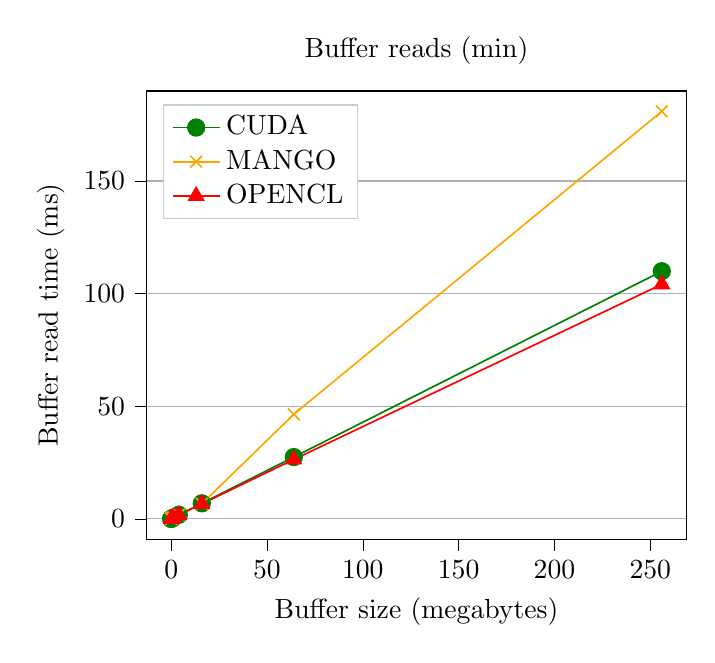
\begin{tikzpicture}

\definecolor{color0}{rgb}{1,0.647058823529412,0}

\begin{axis}[
legend cell align={left},
legend style={
  fill opacity=1,
  draw opacity=1,
  text opacity=1,
  at={(0.03,0.97)},
  anchor=north west,
  draw=white!80!black
},
tick align=outside,
tick pos=left,
title={Buffer reads (min)},
x grid style={white!69.0196078431373!black},
xlabel={Buffer size (megabytes)},
xmin=-12.78359375, xmax=268.79921875,
xtick style={color=black},
y grid style={white!69.0196078431373!black},
ylabel={Buffer read time (ms)},
ymajorgrids,
ymin=-9.03422905142857, ymax=189.990061773878,
ytick style={color=black},
yticklabel style={/pgf/number format/fixed},
]
\addplot [semithick, green!50.1960784313725!black, mark=*, mark size=3, mark options={solid}]
table {%
0.015625 0.0123296224489796
0.0625 0.0205413469387755
0.25 0.130403275862069
1 0.505512620689655
4 1.83742425
16 6.9285274
64 27.4589087
256 109.953671
};
\addlegendentry{CUDA}
\addplot [semithick, color0, mark=x, mark size=3, mark options={solid}]
table {%
0.015625 0.0806020101010101
0.0625 0.16509962
0.25 0.282117206896552
1 0.732995033333333
4 1.89954115
16 6.7418782
64 46.451228
256 180.9435031
};
\addlegendentry{MANGO}
\addplot [semithick, red, mark=triangle*, mark size=3, mark options={solid}]
table {%
0.015625 0.0137764387755102
0.0625 0.02193194
0.25 0.136782633333333
1 0.511125655172414
4 1.78901245
16 6.68551331578947
64 26.398961
256 104.1510284
};
\addlegendentry{OPENCL}
\end{axis}

\end{tikzpicture}
